\subsection{Network layer technologies}
The simplest path discovery algorithm is flooding, where all nodes are peers (flat routing). A sensor node simply broadcast a packet to all of its neighbours, which do the same until a packet reaches the destination. This introduces a problem of the packet circling a network indefinitely, which may be countered by hop count or time to leave field; when the packet is forwarded through a node its hop count is decremented until zero is reached or time to leave is incremented until given number is reached and then it is discarded. Even thought this approach is simple and does not require costly topology or network maintenance it has a drawbacks like traffic implosion (same packet delivered from different nodes to the same one), overlap problem (neighbouring nodes sense similar data info and send them to the same node) or resource blindness (this approach does not care about resource efficiency e.g. power source may be depleted fats).

Gossiping is an approach for path discovery which improve the flooding approach and its shortcomings. In here, the node randomly sends a packet to only one of its neighbours. This way the traffic implosion and overlap problem are overcome. However, it is not suitable for use in extensive networks as this approach explores only one path at the time which would be very time consuming. 

More advanced routing approach is \acrfull{spin}, which is based on negations, as the name already suggest. It faces shortcomings of Flooding and Gossiping namely resource blindness (power source of highly active nodes is depleted quickly), overlapping or performance of network as they grow in size. \acrshort{spin} is data-centric. When a node has a packet to send, there are three steps in the process. First step is an \texttt{ADV} (advertisement) query with metadata sent to all neighbouring nodes, suggesting what data are being send and asking for transmission. Nodes that are willing to receive and re-transmit the data responds with \texttt{REQ} (request) message. Then the node sends \texttt{DATA} (header + metadata + packet) to all nodes that requested those data. So, there are three types of messages in total: \texttt{ADV}, \texttt{REQ} and \texttt{DATA}. The process may be seen in Figure~\ref{fig:spin-protocol}. Data negotiation process happens when the node asks its neighbours (\texttt{ADV}) to send them data and neighbours learns about what data will be send from metadata. Based on the metadata and resource adaptation process (keeps track of power source level and consumption and if the power source level is too low, it will not request the data, which prolongs node’s lifetime) a node decides whether it will request data from the sender or not.

\begin{figure}[ht]
    \centering
    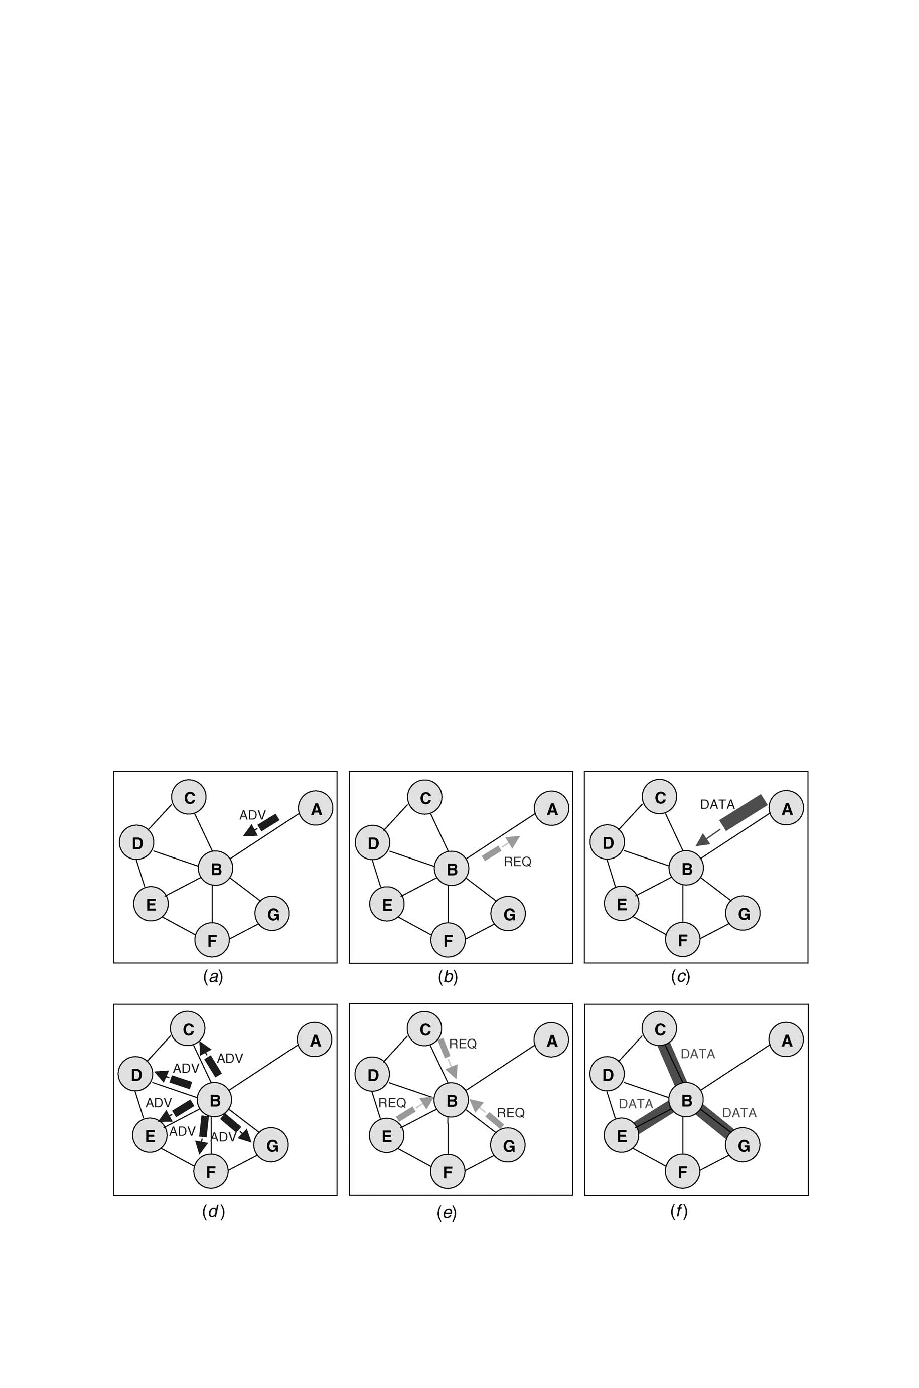
\includegraphics[width=0.8\textwidth]{00images/spin-protocol}
    \caption[itemize]{Operation of the \acrshort{spin} protocol:
    \begin{enumerate*}[label=(\alph*)]
        \item Node A sends ADV query to all its neighbours (B)
        \item Node B receives ADV and decides to accept data, REQ query is send back to node A
        \item Node A sends DATA to node B.
        \item Node B sends ADV query to all its neighbours (C, D, E, F, G)
        \item Nodes C, D, E, F, G receive ADV but only nodes C, E and G decides to accept data and to send REQ query to node A
        \item Node A sends DATA to nodes C, E, G
    \end{enumerate*}
    Figure taken from~\cite{Sohraby2007WirelessApplications}.
    }
    \label{fig:spin-protocol}
\end{figure}

Another approach to routing is \acrfull{leach}, which is based on hierarchical system. Network is divided into clusters with each cluster having a cluster head. The cluster head is responsible of data gathering, its aggregation and transmission to the sink. An assumption is made that each cluster head is one hop from the sink. LEACH has two phases: set-up phase: a cluster head is chosen, and a cluster formed, and steady phase: messages are collected, aggregated and transmitted by a cluster head. This approach achieves significant power saving because of message aggregation and because of master head rotation throughout nodes, all of them are utilised approximately the same. No global information besides who cluster heads are needed as local cluster management is used. Shortcomings of \acrshort{leach} are one-hop assumption from a cluster head to the sink, which is not always true as the cluster head position is rotating and different nodes are at different positions needing more or less power to transmit data to sink when being cluster heads, then choosing a right steady-phase duration is crucial to not deplete one node too much.

\acrfull{pegasus} and hierarchical \acrshort{pegasus} are routing protocols which gather information. They assume that there is a global knowledge of where each node in the network is. \acrshort{pegasus} family uses chain structure. The chain formation is as follows: the furthest node from the sink is selected, then it adjusts its signal strength so that only one neighbour is in reach and makes a connection with it; this way it follows until the sink is reached. For data transmission a chain leader must be chosen (is selected randomly), which is changed every round. Then it gives a token to the rightmost node of the chain from him, which may start sending data down the chain until they reach the chain leader; the same process is then repeated for the leftmost node. When all data are aggregated, the chain leader transmit all data to the sink (it may need to adjust it signal strength to do that) and chain leader is changed. This process is rather slow, and therefore if all nodes are equipped with \acrshort{cdma} transmitter, they may send data to its pair neighbour partner until the chain leader is reached, as it may be seen in Figure~\ref{fig:chain-pegasis}.

\begin{figure}[ht]
    \centering
    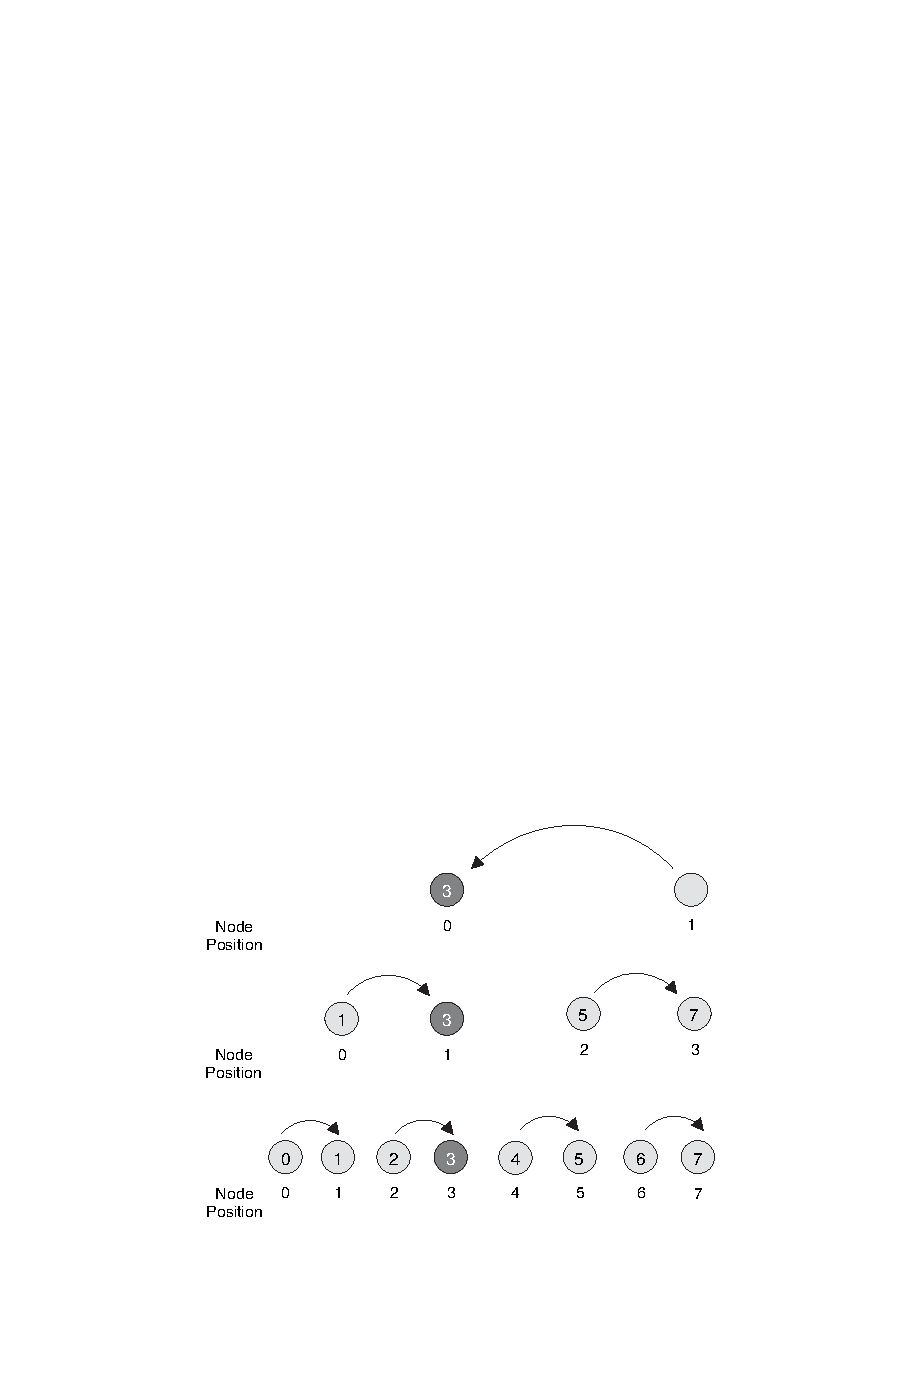
\includegraphics[width=0.8\textwidth]{00images/chain-pegasis}
    \caption{Chain structure of \acrshort{pegasus}. In first step all left nodes in nodes pairs send data to their pair neighbour. This process is repeated and new neighbour pairs are being created as well, until all data are aggregated at the chain leader. Taken from~\cite{Sohraby2007WirelessApplications}}
    \label{fig:chain-pegasis}
\end{figure}

\paragraph{Conclusion}
As may it may have been read at the beginning of this report, our proposed system is made out of two parts: network within a single container and a network on the vessel. Now an analysis of which routing approach or protocol is suitable the most for the given case will be conducted. 
In the case of a network within a container, the most important requirement would be power efficiency. The reason is that sensors within the container are desired to be wireless without cables, neither power cables. Rest of requirements are on the same level, because a delay does not play a big role as long as data are delivered and data to be delivered are not life-threatening, so if it happens that they will not be delivered, nothing happens. There are no more requirements or restrictions than these, so a suggested routing approach is Gossiping. The main reason is the number of sensors within a container which are expected not to be more than to be counted in tens. This suggest rather a smaller wireless sensor network with one sink, where it will not take so long for a packet to be delivered from the sending node to the sink, also it is cheap to produce such sensor.

\acrshort{wsn} on the vessel on the other hand will have more complex structure, and containers within a range of the base station will be constantly changing, and a number of nodes would be counted in thousands. However, power consumption constrains will not be a problem as on the vessel each container will be connected to a power source and so the node’s transmitter. Also, delay and message delivery do not play a big role. The most suitable routing approaches suggested are therefore \acrshort{leach} and \acrshort{pegasus} (with \acrshort{cdma}), as Flooding, Gossiping and \acrshort{spin} are not suitable for networks of this size.

